\documentclass[12pt]{ociamthesis}  % default square logo 
%\documentclass[12pt,beltcrest]{ociamthesis} % use old belt crest logo
%\documentclass[12pt,shieldcrest]{ociamthesis} % use older shield crest logo

%load any additional packages
\usepackage{amssymb}
\usepackage{listings}

\usepackage{color}
 
\definecolor{codegreen}{rgb}{0,0.6,0}
\definecolor{codegray}{rgb}{0.5,0.5,0.5}
\definecolor{codepurple}{rgb}{0.58,0,0.82}
\definecolor{backcolour}{rgb}{0.95,0.95,0.92}
 
\lstdefinestyle{mystyle}{
    backgroundcolor=\color{backcolour},   
    commentstyle=\color{codegreen},
    keywordstyle=\color{magenta},
    numberstyle=\tiny\color{codegray},
    stringstyle=\color{codepurple},
    basicstyle=\footnotesize,
    breakatwhitespace=false,         
    breaklines=true,                 
    captionpos=b,                    
    keepspaces=true,                 
    numbers=left,                    
    numbersep=5pt,                  
    showspaces=false,                
    showstringspaces=false,
    showtabs=false,                  
    tabsize=2,
    language=python
}
 
\lstset{style=mystyle}
%input macros (i.e. write your own macros file called mymacros.tex 
%and uncomment the next line)
%\include{mymacros}

\title{Modul Praktikum \\[1ex]     %your thesis title,
        Kecerdasan Buatan}   %note \\[1ex] is a line break in the title

\author{Eni Lestari}             %your name
\college{1194012\\[5ex]
Informatics Engineering}  %your college

%\renewcommand{\submittedtext}{change the default text here if needed}
\degree{Politeknik Pos Indonesia}     %the degree
\degreedate{Bandung 2022}         %the degree date

%end the preamble and start the document
\begin{document}

%this baselineskip gives sufficient line spacing for an examiner to easily
%markup the thesis with comments
\baselineskip=18pt plus1pt

%set the number of sectioning levels that get number and appear in the contents
% \setcounter{secnumdepth}{3}
% \setcounter{tocdepth}{3}


\maketitle                  % create a title page from the preamble info
% \include{section/dedication}        % include a dedication.tex file
% \include{section/acknowlegements}   % include an acknowledgements.tex file
% \include{section/abstract}          % include the abstract

\begin{romanpages}          % start roman page numbering
    \tableofcontents            % generate and include a table of contents
    \listoffigures              % generate and include a list of figures
\end{romanpages}            % end roman page numbering

%now include the files of latex for each of the chapters etc
\chapter{Sejarah dan Perkembangan Kecerdasan Buatan}
Buku umum teori lengkap yang digunakan memiliki Semakin maju nya teknologi membuat banyak sekali perangkat pintar yang kemudian mengadopsi teknologi Kecerdasan buatan atau biasa disebut dengan Artificial Intelligence (AI). Dengan adanya kehadiran AI ini menimbulkan banyak sekali manfaat tentunya, ia dapat meringankan beban pekerjaan masuia serta membuatnya lebih efektif dan juga efisien. Kecerdasan buatan dapat disimpulkan sebagai suatu kecerdasan atau keahlian yang pada dasarnya merupakan buatan manusia. Yang mana kecerdasan otak manusia itu ialah alami dimiliki dan tumbuh sepanjang seseorang tersebut bernafas. Setelah itu, seseorang dengan kecerdasan alami ini lah kemudian mulai merangkai sebuah sistem atau perangkat, yang bertujuan supaya perangkat ini dapat memudahkan suatu pekerjaan sendiri maupun orang lain dalam tanda kutip manusia. Untuk alat yang berhasil diciptakan dan teknologi yang berhasil dilahirkan inilah yang kemudian disebut sebagai AI.
Pada awalnya ai mulai dikenal publik itu karena ia memiliki kemampuan baik dalam menitu kegiatan manusia. Yang kemudian memunculkan banyak anggapan negetif, dimana manusia akan digeser oleh mesin. Akan tetapi semakin berkembangnya waktu, anggapan itupun berubah menjadi anggapan positif, karena dengan adanya AI ini dapat mempermudah dan mempuat pekerjaan menjadi mudah, cepat dan juga efektif efisien. Dengan adanya AI ini  dinilai dapat membantu pekerjaan sehari-hari dan juga mudah untuk dikendalikan. Yang kemudian AI sudah dijadikan sebagai teman dan bukan lagi dianggap sebagai musuh atau pun ancaman bagi manusia.


Adapun manfaat dari teknologi AI ini antara lain sebagai berikut :
\begin{enumerate}
	\item
	      Membantu meminimalkan kesalahan
	\item
	      Solusi untuk hemat energi
	\item
	      Berperan dalam eksplorasi kekayaan alam
	\item
	      Hemat SDM
	\item
	      Bermanfaat di bidang kesehatan
\end{enumerate}

\section{Supervised Learning}
Supervised Learning adalah tugas pengumpulan data untuk menyimpulkan fungsi dari data pelatihan berlabel. Data pelatihan terdiri dari serangkaian contoh pelatihan. Dalam supervised learning, setiap contoh adalah pasangan yang terdiri dari objek input (biasanya vektor) dan nilai output yang diinginkan(juga disebut sinyal pengawasan super). Algoritma pembelajaran yang diawasi menganalisis data pelatihan dan menghasilkan fungsi yang disimpulkan, yang dapat digunakan untuk memetakan contoh-contoh baru.Supervised Learning menyediakan algoritma pembelajaran dengan jumlah yang diketahui untuk mendukung penilaian dimasa depan. Chatbots, mobil self-driving, program pengenalan wajah, sistem pakar dan robot adalah beberapa sistem yang dapat menggunakan pembelajaran yang diawasi atau tidak. Model Supervised Learning memiliki beberapa keunggulan dibandingkan pendekatan tanpa pengawasan, tetapi mereka juga memiliki keterbatasan. Sistem lebih cenderung membuat penilaian bahwa manusia dapat berhubungan, misalnya karena manusia telah memberikan dasar untuk keputusan. Namun, dalam kasus metode berbasis pengambilan, Supervised Learning mengalami kesulitan dalam menangani informaasi baru. Jika suatu sistem dengan kategori untuk mobil dan truk disajikan dengan sepeda, misalnya ia harus salah dikelompokkan dalam satu kategori ata yang lain. Namun. jika sistem AI bersifat generatif, ia mungkin tidak tahu apa sepeda itu tetapi akan dapat mengenalinya sebagai milik kategori yang terpisah

\section{Klasifikasi dan Regresi}
Klasifikasi yaitu pendekatan pembelajaran yang diawasi dimana program komputer belajar dari input data yag diberikan  kepadanya dan kemudian menggunakan pembelajaran ini untuk mengklarifikasikan pengamatan baru. Regresi adalah membehas mengenai masalah ketika variable output adalah nilai rill atau berkelanjutan contohnya seperti "gaji" atau "berat". banyak model yang berbeda dapat digunakan makan, yang paling sederhana adalah regresi linier. ia mencoba untuk menyesuaikan data degan hyper-plane terbaik yang melewati poin.

\section{Unsupervised Learing}
Unsupervised Learning berbeda dengan Supervised Leraning. Perbedaannya ialah unsupervised learning tidak memiliki data latih, sehingga dari data yang ada kita mengelompokan data tersebut menjadi 2 ataupun 3 bagian dan seterusnya. Unsupervised Learning adalah pelatihan algoritma kecerdasan buatan (AI) menggunakan informasi yang tidak diklasifikasikan atau diberi label dan memungkinkan algoritma untuk bertindak atas informasi tersebut tanpa bimbingan.
Dalam Unsupervised Learning, sistem AI dapat mengelompokkan informasi yang tidak disortir berdasarkan persamaan dan perbedaan meskipun tidak ada kategori yang disediakan

\section{Data set, Traning set, Testing set}
Dataset adalah objek yang merepresentasikan data dan juga relasi yang ada di memory. Strukturnya mirip dengan data di database, namun bedanya dataset berisi koleksi dari data table dan data relation. Training Set adalah set digunakan oleh algoritma klassifikasi . Dapat dicontohkan dengan : decision tree, bayesian, neural network dll. Testing Set adalah set yang digunakan untuk mengukur sejauh mana classifier berhasil melakukan klasifikasi dengan benar. Ini berfungsi sebagai meterai persetujuan, dan Anda tidak menggunakannya sampai akhir.
% \include{section/chapter2}
% \chapter{Prediksi dengan Random Forest}

Random forest adalah suatu algoritma yang digunakan pada klasifikasi data dalam jumlah yang besar. Proses klasifikasi pada random forest berawal dari memecah data sampel yang ada kedalam decision tree secara acak. Setelah pohon terbentuk,maka akan dilakukan voting pada setiap kelas dari data sampel. Kemudian, mengkombinasikan vote dari setiap kelas kemudian diambil vote yang paling banyak.Random forest terdiri dari kumpulan decision tree. Random forest merupakan algoritma supervised learning yang digunakan untuk klasifikasi dan regresi. Random forest dapat menangani kumpulan data yang berisi variable kontinu seperti dalam kasus regresi dan variable kategoris dalam kasus klasifikasi. Random forest bekerja sepeti enseble dimana enseble berarti menggabungkan beberapa model menjadi kumpulan model yang digunakan untuk membuat prediksi. Random forest akan memilih pengamatan secara acak kemudian membangun sebuah decision tree dan mengambil hasil rata-ratanya.

\section{Dataset}
Dataset adalah sekumpulan data yang disusun secara terstruktur. Biasanya, dataset dipresentasikan dalam bentuk tabel, alias baris dan kolom. Dataset merupakan sekumpulan data dimana data terabut berasal dari informasi di masa lalu yang dikelola menjadi sebuah informasi untuk dapat melakukan data mining. Dataset berisi lebih dari satu variable yang digunakan untuk klasifikasi. Cara Membaca Dataset dan Arti Setiap File dan isi Field Masing-masing File :
\begin{enumerate}
    \item Langkah awal yaitu dengan Menggunakan library Pandas pada python untuk membaca dataset dengan format text file.
    \item Selanjutnya buat variable baru misalnya "dataset" yang berisi perintah untuk membaca file dataset.
\end{enumerate}

\section{Cross Validation}
Cross Validation adalah metode yang paling biasa digunakan untuk evaluasi kinerja prediktif dari model. Data biasanya dibagi menjadi dua bagian dan berdasarkan pemisahan ini pada satu bagian, pelatihan dilakukan sementara prediktif diuji pada bagian lain. Cross validation merupakan metode untuk mengevaluasi dan membandingkan algoritma dengan membagi data menjadi dua yaiti data latih dan data uji. Cross validation (CV) adalah salah satu teknik yang digunakan untuk menguji keefektifan suatu model dan merupakan prosedur pengambilan sampel ulang yang digunakan untuk mengevaluasi suatu model jika memiliki data yang terbatas. Untuk dapat melakukan CV maka perlu menyisihkan sampel/sebagian data yang tidak digunakan untuk melatih model, kemudian menggunakan sampel ini untuk pengujian/validasi. Bentuk dasar dari cross-validation adalah k-fold cross-validation.

\section{Arti Score 44\% Pada Random Forest, 27\% Pada Decission Tree Dan 29\% Dari SVM}
merupakan presentase keakurasian prediksi yang dilakukan pada saat testing
menggunakan label pada dataset yang digunakan. Score akan mendefinisikan
aturan evaluasi model, kemudian saat dijalankan akan muncul sebuah persentase yang menunjukan keakurasian atau keberhasilan dari prediksi yang dilakukan. Jika
menggunakan Random Forest maka hasilnya 40\% dan jika menggunakan Decission Tree hasil prediksinya yaitu 27\% dan pada SVM 29\%.

\section{Confusion Matrix}
Confusion Matrix adalah pengukuran performa untuk masalah klasifikasi machine learning dimana keluaran dapat berupa dua kelas atau lebih. Confusion Matrix adalah tabel dengan 4 kombinasi berbeda dari nilai prediksi dan nilai aktual. Confusion Matrix atau disebut juga dengan Error Matrix pada dasarnya akan memberikan informasi mengenai perbandingan hasil dari klasifikasi yang dilakukan oleh model atau sistem dengan hasil sebenarnya. Confusion Matrix berbentuk tabel matrix yang akan menggambarkan kinerja dari model klasifikasi pada data uji yang nilai sebenarnya diketahui.
\newline
\textbf {Berikut adalah contoh dari confusion matrix :}
\begin{enumerate}
    \item Precision (Positive Predictive Value)
    \item Accuracy
    \item Recall atau Sensitivity (True Positive Rate)
\end{enumerate}
\textbf {Langkah membuat dan membaca confusion matrix}
\begin{enumerate}
    \item Langkah awal yaitu Tentukan pokok permasalahan atau menggunakan dataset, misalnya data pasien covid
    \item Langkah selanjutnya, Membagi dataset serta membuat model prediksi menggunakan Decision Tree. Dataset dibagi menjadi dua yaitu data latiih dan data uji. Data latih digunakan untuk melatih model yang dibuat dan evaluasi akan dilakukan pada data uji.
    \item lalu langkah terkahir, Evaluasi model menggunakan confusion matrix yaitu untuk mengetahui keakuratan model yang sudah dibuat menggunakan performance metrics seperti: accuracy, recall, dan precision.
\end{enumerate}

\section{Voting Pada Random Forest}
Target prediksi dengan voting tertinggi digunakan sebagai prediksi akhir dari algoritma random forest. Voting merupakan suara untuk setiap target yang diprediksi pada saat melakukan Random Forest.

\section{Praktikum}
\subsection{Aplikasi Sederhana Menggunakan Pandas}
\begin{figure}[!htbp]
    \centering

    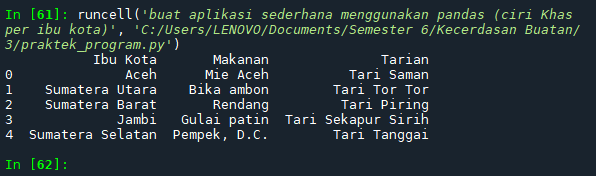
\includegraphics[width=10cm,height=4cm]{figures/Cp3-1.png}
    \caption{Aplikasi sederhana menggunakan pandas}
    \label{penanda}
\end{figure}
\textbf{Penjelasan Code Aplikasi Sederhana pandas perbaris :}
\begin{itemize}
    \item Langkah awal yaitu di line 1 merupakan langkah mengimport library pandas kemudian di inisialisasi menjadi pd
    \item Untuk bagian Variable data di definisikan data data untuk kolom nama, kolom npm dan kolom angkatan
    \item Pada bagian Variable frame itu akan berfungsi mengubah data pada variable data disejajarkan dengan baris dan kolom menggunakan pd dataframe
    \item Selanjutnya Peritah frame kemudian dijalankan untuk dapat menampilkan hasil dari dataframe
\end{itemize}

\subsection{Aplikasi Sederhana Menggunakan Matplotlib}
\begin{figure}[!htbp]
    \centering
    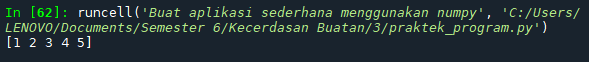
\includegraphics[width=10cm,height=2cm]{figures/Cp3-2.png}
    \caption{Aplikasi sederhana menggunakan matplotlib}
    \label{penanda}
\end{figure}
\textbf{Penjelasan Code Aplikasi Sederhana matplotlib perbaris :}
\begin{itemize}
    \item Baris Pertama Yaitu import library matplotlib kemudian di inisialisasi menjadi plt
    \item Variable prodi sebagai sumbu x untuk nama nama prodi
    \item Variable jumlah mhs sebagai sumbu y untuk jumlah atau banyaknya mahasiswa
    \item plt figure digunakan untuk mengatur size dan plt bar merupakan fungsi yang digunakan untuk memvisualisasikan bar
    \item plt title digunakan untuk memberikan judul dan plt ylabel untuk memberikan judul pada sumbu y
    \item plt yticks dan xticks digunakan untuk mengatur size tulisan pada sumbu y dan x
\end{itemize}

\subsection{Aplikasi Sederhana Menggunakan Numpy}
\begin{figure}[!htbp]
    \centering
    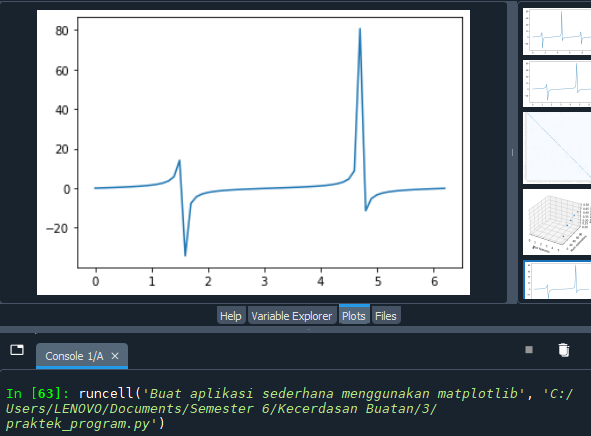
\includegraphics[width=6cm,height=6cm]{figures/Cp3-3.png}
    \caption{Aplikasi sederhana menggunakan numpy}
    \label{penanda}
\end{figure}
\textbf{Penjelasan Code Aplikasi Sederhana numpy perbaris :}
\begin{itemize}
    \item Baris Pertama Yaitu import library numpy kemudian di inisialisasi menjadi np
    \item Variable a digunakan sebagi fungsi array yang pertama
    \item Variable b digunakan sebagai fungsi array yang kedua
    \item Variable c digunakan sebagai fungsi array yang ketiga
    \item Perintah print digunakan untuk menampilkan hasil array
    \item Operasi pada array menggunakan perkalian pada a dan b dan penjumlahan pada b dan c
\end{itemize}


\section{Program Klasifikasi Random Forest}
Berikut merupakan output dari percobaan Random Forest yang telah dilakukan :
\begin{enumerate}

    \begin{figure}[!htbp]
        \centering
        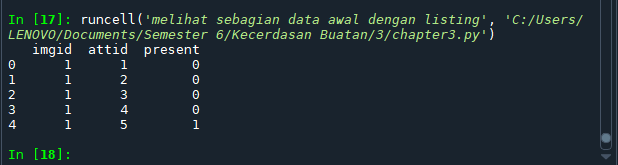
\includegraphics[width=12cm,height=6cm]{figures/Cp3-4.png}
        \caption{Membaca dataset file txt}
        \label{penanda}
    \end{figure}

    \item Kode berikut akan menampilkan output banyaknya jumlah baris dan kolom data frame imgatt
          \begin{figure}[!htbp]
              \centering
              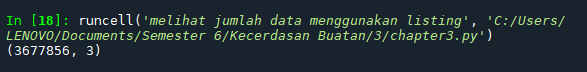
\includegraphics[width=4cm,height=1cm]{figures/Cp3-5.png}
              \caption{Mengetahui jumlah data}
              \label{penanda}
          \end{figure}

    \item imgatt2 menggunakan function pivot untuk merubah kolom menjadi baris dan baris menjadi kolom dari data frame sebelumnya.
          \begin{figure}[!htbp]
              \centering
              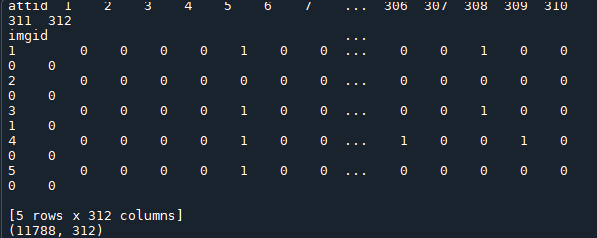
\includegraphics[width=12cm,height=2cm]{figures/Cp3-6.png}
              \caption{Pivot dataset}
              \label{penanda}
          \end{figure}

    \item Pada kode berikut digunakan dataset label kemudian akan diberi label pada burung dan menentukan burung tersebut ke dalam spesies apa. di dalam data yang sebelumnya ada 312 kolom dimana 312 data tersebut memiliki kelompoknya masing-masing. Dalam hal ini akan dimunculkan dua kolom pada variable explorer yaitu imgd dan label yang terdiri dari 11788 baris dan 1 kolom
          \begin{figure}[!htbp]
              \centering
              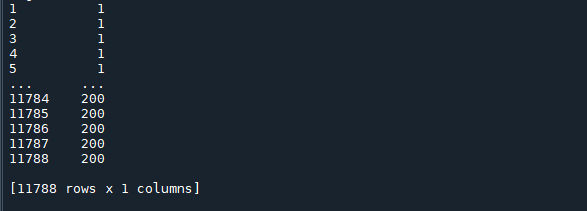
\includegraphics[width=12cm,height=2cm]{figures/Cp3-7.png}
              \caption{Membaca Dataset label}
              \label{penanda}
          \end{figure}

    \item Selanjutnya data imgatt2 akan join dengan imglabels atau menggabungkan field dari dua file yang terpisah, karena data baris sama banyak nya maka ditambahkan data kolom dari imgatt2 312 kolom dengan imglabels 1 kolom, maka hasilnya menjadi 313 kolom
          \begin{figure}[!htbp]
              \centering
              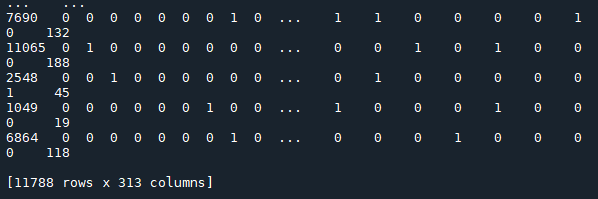
\includegraphics[width=7cm,height=2cm]{figures/Cp3-8.png}
              \caption{Menggabungkan field dari file yang terpisah}
              \label{penanda}
          \end{figure}

    \item Kemudian memisahkan dan memilih label atau memecah data kembali seperti sebelumnya dengan cara mengambil 312 dari belakang dan mengambil 312 dari depan.
          \begin{figure}[!htbp]
              \centering
              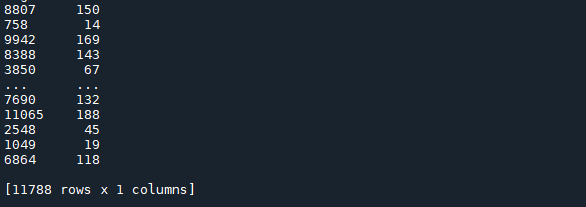
\includegraphics[width=7cm,height=2cm]{figures/Cp3-9.png}
              \caption{Memisahkan dan memilih label}
              \label{penanda}
          \end{figure}

    \item Membagi Data training dan data testing dengan mengambil row sebanyak 8000 dari akhir untuk training dan 8000 dari awal untuk data testing.
          \begin{figure}[!htbp]
              \centering
              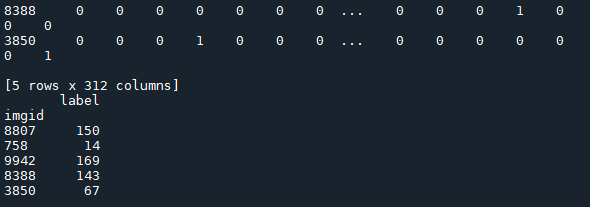
\includegraphics[width=7cm,height=3cm]{figures/Cp3-10}
              \caption{Pembagian data training dan tes}
              \label{penanda}
          \end{figure}

    \item Melakukan klasifikasi, di dalam kelas randomforestclassifier setting parameter variable yaitu 50 dalam satu independen tree maksimal akan mengakomodir 50 atribut. Kemudian lakukan instansiasi dengan melakukan klasifikasi pada data train att beserta data label nya.
          \begin{figure}[!htbp]
              \centering
              
\includegraphics[width=14cm,height=3cm]{figures/Cp3-11}
              \caption{Instansiasi kelas Random Forest}
              \label{penanda}
          \end{figure}
\end{enumerate}

\section{Program Confusion Matrix}
Berikut merupakan output dari percobaan Confusion Matrix yang telah dilakukan :
\begin{enumerate}

    \item Selanjutnya plotting confusion matrix menggunakan matplotlib.
          \begin{figure}[!htbp]
              \centering
              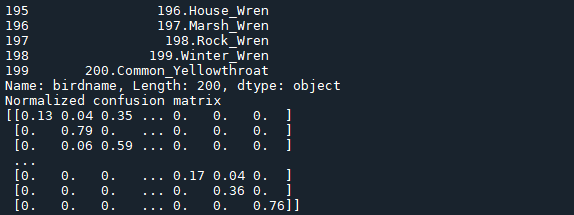
\includegraphics[width=11cm,height=11cm]{figures/Cp3-12.png}
              \caption{Plotting Confusion Matrix}
              \label{penanda}
          \end{figure}

    \item Membaca File Classes
          \begin{figure}[!htbp]
              \centering
              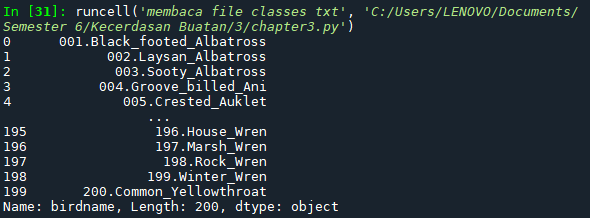
\includegraphics[width=11cm,height=5cm]{figures/Cp3-13.png}
              \caption{Membaca file classes}
              \label{penanda}
          \end{figure}

    \item Plot hasil perubahan label
          \begin{figure}[!htbp]
              \centering
              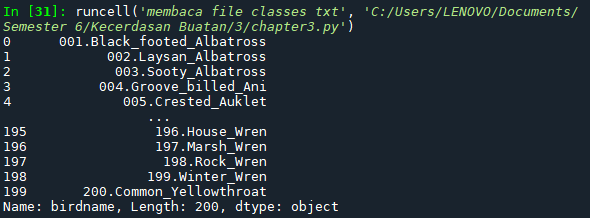
\includegraphics[width=10cm,height=4cm]{figures/Cp3-14.png}
              \caption{Plot hasil perubahan label}
              \label{penanda}
          \end{figure}
\end{enumerate}


\section{Program Klasifikasi SVM dan Decission Tree}
Berikut merupakan output dari percobaan Klasifikasi SVM dan Decission Tree yang telah dilakukan :
\begin{enumerate}
    \begin{figure}[!htbp]
        \centering
        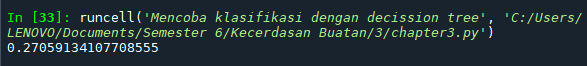
\includegraphics[width=8cm,height=2cm]{figures/Cp3-15.png}
        \caption{Klasifikasi Decission Tree}
        \label{penanda}
    \end{figure}

    \item Klasifikasi SVM dengan menggunakan dataset yang sama
          \begin{figure}[!htbp]
              \centering
              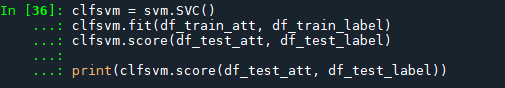
\includegraphics[width=8cm,height=2cm]{figures/Cp3-16.png}
              \caption{Klasifikasi SVM}
              \label{penanda}
          \end{figure}
\end{enumerate}

\section{Program Cross Validation}
Berikut merupakan output dari percobaan Program Cross Validation yang telah dilakukan :
\begin{enumerate}
    \item tugas minggu hari ini dan besok (maks 100). pada chapter ini
    \item presentasi decission tree (maks 100). Mempraktekkan kode python dan menjelaskan cara kerjanya.
    \item presentasi Random Forest (maks 100).Mempraktekkan kode python dan menjelaskan cara kerjanya.
    \item Hasil Cross Validation untuk Random forest
          \begin{figure}[!htbp]
              \centering
              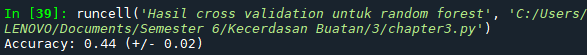
\includegraphics[width=14cm,height=2cm]{figures/Cp3-17.png}
              \caption{Hasil Cross Validation Random Forest}
              \label{penanda}
          \end{figure}
    \item Hasil Cross Validation untuk Decission Tree
          \begin{figure}[!htbp]
              \centering
              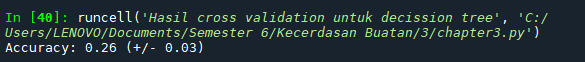
\includegraphics[width=14cm,height=1cm]{figures/Cp3-18.png}
              \caption{Hasil Cross Validation Decission Tree}
              \label{penanda}
          \end{figure}
    \item Hasil Cross Validation untuk SVM
          \begin{figure}
              \centering
              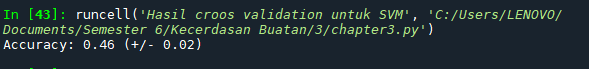
\includegraphics[width=14cm,height=1cm]{figures/Cp3-19.png}
              \caption{Hasil Cross Validation SVM}
              \label{penanda}
          \end{figure}
\end{enumerate}

\section{Program Pengamatan Komponen Informasi}
Berikut merupakan output dari percobaan Program Pengamatan Komponen Informasi yang telah dilakukan :
\begin{enumerate}
    \item Ouput berikut dapat mengetahui banyaknya tree yang dibuat, berapa atribut yang digunakan dan informasi lainnya.
          \begin{figure}
              \centering
              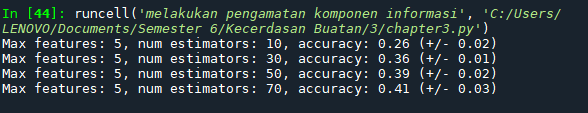
\includegraphics[width=11cm,height=5cm]{figures/Cp3-20.png}
              \caption{Hasil plotting komponen}
              \label{penanda}
          \end{figure}
    \item Output berikut merupakan hasil plotting komponen informasi agar dapat dibaca
          \begin{figure}
              \centering
              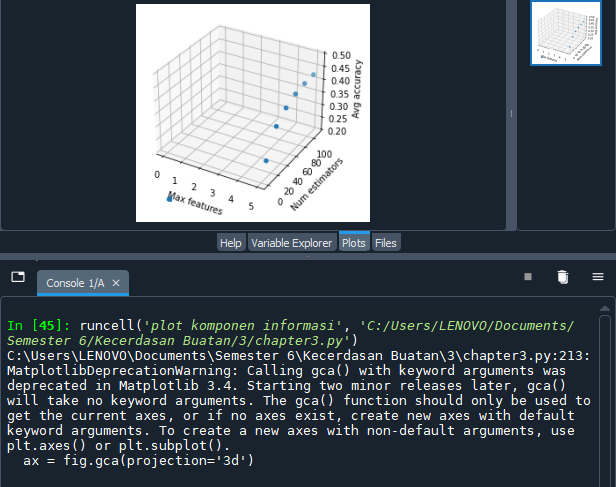
\includegraphics[width=8cm,height=9cm]{figures/Cp3-21.png}
              \caption{Hasil plotting komponen}
              \label{penanda}
          \end{figure}
\end{enumerate}
% \chapter{Klasifikasi Teks}

\section{Klasifikasi Teks}
Merupakan suatu cara dalam memilah milah data teks berdasarkan pada parameter dengan data yang bersifat dokumen ataupun teks yang memiliki kumpulan teks didalamnya, Untuk tipe data teks sendiri yaitu bertipe data char dan string yang mudah untuk diolah

\section{Klasifikasi bunga tidak dapat menggunakan machine learning}
Karena memiliki masalah input yang sama namun keluarannya berbeda (output), jika terjadi error pada inputan maka disebut dengan ‘noise’. Noise sendiri merupakan suatu output yang disimpan/ditangkap maupun direkap bukan seperti seharusnya (keluaran yang diinginkan).

\section{Teknik pembelajaran mesin pada teks pada kata-kata yang digunakan di youtube }
Pada saat menggunakan Youtube terdapat Machine Learning yang bekerja dan memproses perintah
ataupun aktivitas tersebut, dimana akan memfilter secara otomatis video yang disesuaikan
dengan "keyword" yang kita masukkan sehingga memberikan keluaran video dengan keyword yang benar. Adapula fitur yang didapatkan ketika sedang menonton youtube. Pada tampilan sebelah kanan terdapat pilihan 'Next' ataupun 'Suggestion' yang menampilkan video serupa sesuai dengan kita cari atau sedang di tonton.

\section{Vektorisasi Data}
Vektorisasi data adalah proses normalisasi data teks dengan pemberian nilai terhadap setiap fitur. Pada penelitian ini digunakan teknik TF-IDF untuk pemberian bobot fitur. Teknik ini akan menghitung nilai Term Frequency (TF) dan Inverse Document Frequency (IDF) pada setiap fitur di setiap dokumen dalam korpus

\section{Bag-of-words}
Bag-of-words merupakan suatu representasi penyederhanaan yang digunakan dalam suatu pemrosesan Bahasa alami dan dapat mengambil informasi. Model bag-of-words sederhana untuk dipahami dan diterapkan dan juga dapat diandalkan dalam menangani masalah pemodelan Bahasa dan klasifikasi dokumen. Pada model ini, tiap kalimat dalam dokumen digambarkan sebagai token

\section{TFIDF}
tf–idf, TF*IDF, atau TFIDF adalah ukuran statistik yang menggambarkan pentingnya suatu istilah terhadap sebuah dokumen dalam sebuah kumpulan atau korpus. Ukuran ini sering dipakai sebagai faktor pembobot dalam pencarian temu balik informasi, penambangan teks, dan pemodelan pengguna.


\section{Praktikum}
\subsection{Aplikasi Sederhana Menggunakan Pandas}
\begin{figure}[!htbp]
	\centering

	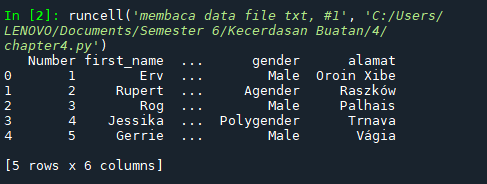
\includegraphics[width=10cm,height=4cm]{figures/Cp4-1.png}
	\caption{Aplikasi sederhana menggunakan pandas}
	\label{penanda}
\end{figure}
\textbf{Penjelasan Code Aplikasi Sederhana pandas perbaris :}
\begin{itemize}
	\item Langkah awal yaitu di line Pertama merupakan langkah mengimport library pandas kemudian di inisialisasi menjadi pd
	\item Untuk bagian Variable data di definisikan data data untuk kolom nama, kolom npm dan kolom angkatan
	\item Lalu membuat variabel dengan nama data dan mengisinya dengan data dummy yang sudah dibuat
	\item Selanjutnya dilihat 5 baris pertama dan banyaknya baris data
\end{itemize}

\subsection{Praktek dataframe tersebut dipecah menjadi dua dataframe yaitu 450 row pertama dan 50 row sisanya}
\begin{figure}[!htbp]
	\centering
	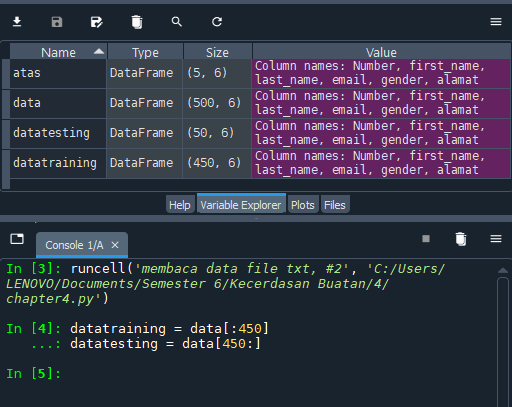
\includegraphics[width=10cm,height=2cm]{figures/Cp4-2.png}
	\caption{Vektorisasi dan Klasifikasi data}
	\label{penanda}
\end{figure}
\textbf{Penjelasan Code hasil pemecahan data perbaris :}
\begin{itemize}
	\item Membuat 2 buah data frame yang pertama 450 data dan yang kedua 50 data
	\item data tersebut terdapat data training dan data testing
\end{itemize}

\subsection{vektorisasi dan klasifikasi dari data (NPM mod 4, jika 0 maka katty
	perry, 1 LMFAO, 2 Eminem, 3 Shakira) dengan Decission Tree}
\begin{figure}[!htbp]
	\centering
	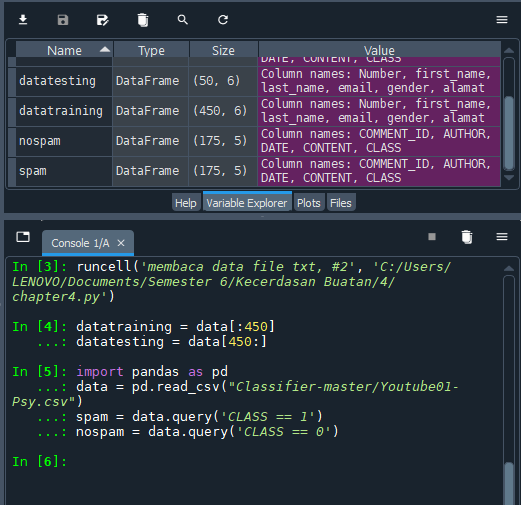
\includegraphics[width=6cm,height=6cm]{figures/Cp4-3.png}
	\caption{Vektorisasi dan Klasifikasi data}
	\label{penanda}
\end{figure}
\textbf{Penjelasan Code Aplikasi Sederhana numpy perbaris :}
\begin{itemize}
	\item Baris Pertama Yaitu import library pandas kemudian di inisialisasi menjadi pd
	\item Melakukan fungsi bag of word dengan cara menghitung semua kata
	\item Melakukan bag of word pada dataframe pada colom CONTENT
	\item Melihat isi vektorisasi
	\item Menampilkan isi data pada baris ke 300
	\item Mengambil apa saja nama kolom yang tersedia
	\item Melakukan randomisasi agar hasil sempurna pada klasifikasi
	\item Membuat data training dan testing
	\item melakukan training pada data training dan di vektorisasi
	\item melakukan testing pada data testing dan di vektorisasi
	\item Dimana akan mengambil label span dan bukan spam
\end{itemize}

\subsection{klasifikasikan dari data vektorisasi dengan klasifikasi SVM}
\begin{figure}[!htbp]
	\centering
	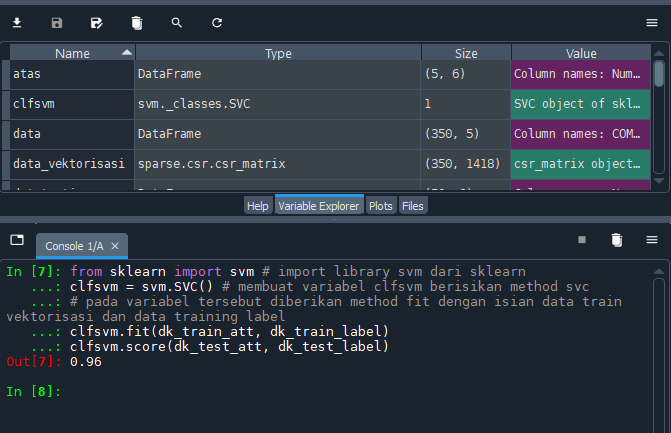
\includegraphics[width=6cm,height=6cm]{figures/Cp4-4.png}
	\caption{Vektorisasi dan Klasifikasi data dengan klasifikasi SVM}
	\label{penanda}
\end{figure}
\textbf{Penjelasan Code klasifikasikan dari data vektorisasi dengan klasifikasi SVM perbaris :}
\begin{itemize}
	\item Baris Pertama Yaitu import library svm dari sklear
	\item membuat variabel clfsvm berisikan method svc
	\item pada variabel tersebut diberikan method fit dengan isian data train vektorisasi dan data training label
\end{itemize}

\subsection{klasifikasikan dari data vektorisasi dengan klasifikasi Decission Tree}
\begin{figure}[!htbp]
	\centering
	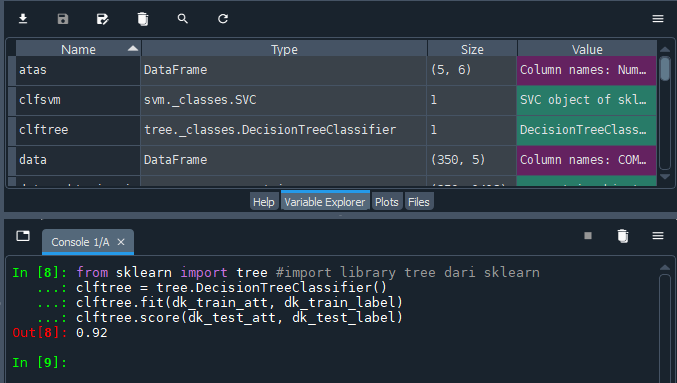
\includegraphics[width=6cm,height=6cm]{figures/Cp4-5.png}
	\caption{Vektorisasi dan Klasifikasi data dengan klasifikasi Decission Tree}
	\label{penanda}
\end{figure}
\textbf{Penjelasan Code klasifikasikan dari data vektorisasi dengan klasifikasi Decission Tree perbaris :}
\begin{itemize}
	\item Baris Pertama Yaitu import library tree dari sklearn
\end{itemize}

\subsection{Plot confusion matrix menggunakan matplotlib}
\begin{figure}[!htbp]
	\centering
	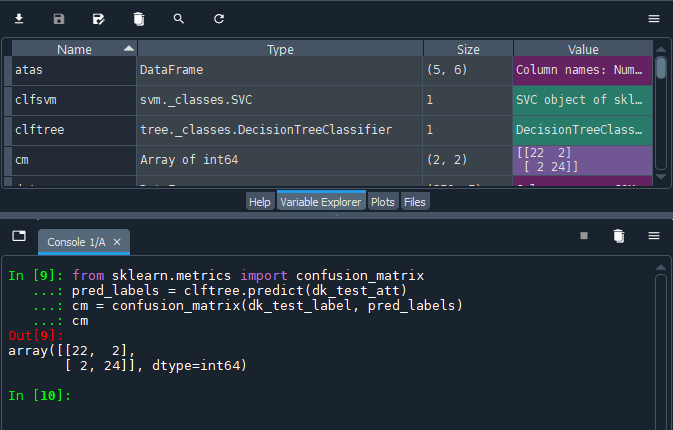
\includegraphics[width=6cm,height=6cm]{figures/Cp4-6.png}
	\caption{Plot confusion matrix menggunakan matplotlib}
	\label{penanda}
\end{figure}
\textbf{Penjelasan Code Plot confusion matrix menggunakan matplotlib perbaris :}
\begin{itemize}
	\item Baris Pertama Yaitu import library confusion matrix dari sklearn metrics
	\item lalu dipanggil lagi cm yaitu confusion matrix yang didalamnya ada dktest label dan pred labels
\end{itemize}

\subsection{Program Cross Validation}
\begin{figure}[!htbp]
	\centering
	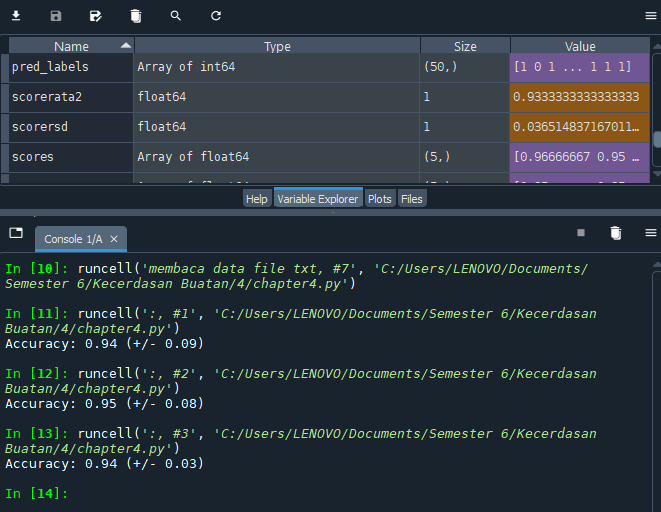
\includegraphics[width=6cm,height=6cm]{figures/Cp4-7.png}
	\caption{Program Cross Validation}
	\label{penanda}
\end{figure}
\textbf{Penjelasan Program Cross Validation perbaris :}
\begin{itemize}
	\item Baris Pertama Yaitu import library cross val score dari sklearn model selection
	\item Lalu menampilkan hasil dari scores
	\item Selanjutnya menampilkan hasil dari scores tree
	\item Dan terakhir itu menampilkan hasil dari scoressvm
\end{itemize}

\subsection{Program Pengamatan Komponen Informasi}
\begin{figure}[!htbp]
	\centering
	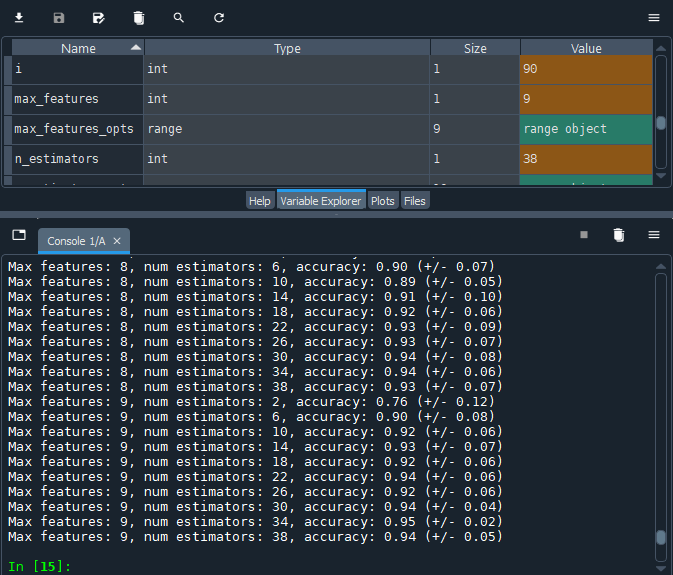
\includegraphics[width=6cm,height=6cm]{figures/Cp4-8.png}
	\caption{Program Pengamatan Komponen Informasi}
	\label{penanda}
\end{figure}
\textbf{Penjelasan Program Pengamatan Komponen Informasi perbaris :}
\begin{itemize}
	\item Baris Pertama Yaitu import numpy yang diinisialisasikan menjadi np
	\item import library RandomForestClassifier dari sklearn ensemble
\end{itemize}

\subsection{Gambar Hasil Akhir}
\begin{figure}[!htbp]
	\centering
	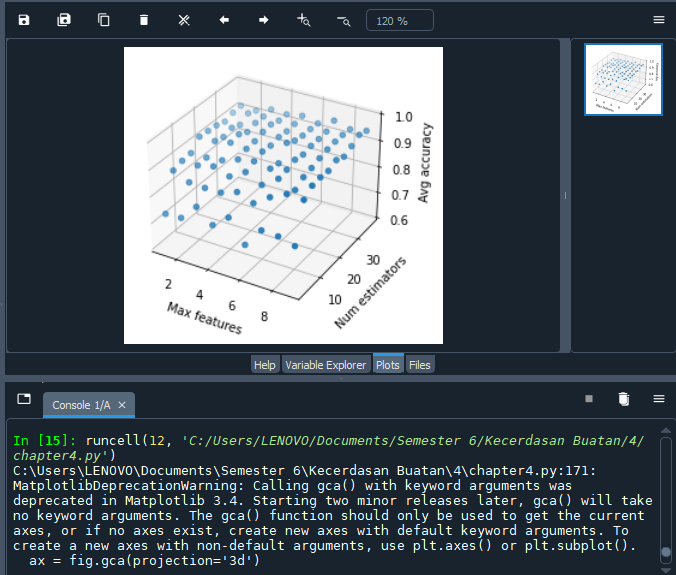
\includegraphics[width=6cm,height=6cm]{figures/Cp4-9.png}
	\caption{Gambar Hasil akhir chapter 4}
	\label{penanda}
\end{figure}
\textbf{Penjelasan Gambar Hasil akhir chapter 4 perbaris :}
\begin{itemize}
	\item Baris Pertama Yaitu import matplotlib pyplot yang diinisialisasikan menjadi plt
	\item import library Axes3D dari mpl toolkits mplot3d
	\item import cm dari matplotlib
	\item lalu disesuaikan ukuran dan juga letak (posisi) untuk gambarnya nanti. 
	\item Selanjutnya atur bagian posisi xyz
	\item lalu show (menampilkan gambar)
\end{itemize}

% \include{section/chapter5}
% \include{section/chapter6}
% \include{section/chapter7}
% \include{section/chapter8}
% \include{section/chapter9}
% \include{section/chapter10}
% \include{section/chapter11}
% \include{section/chapter12}
% \include{section/chapter13}
% \include{section/chapter14}

% %now enable appendix numbering format and include any appendices
% \appendix
% % \include{section/appendix1}
% % \include{section/appendix2}

% %next line adds the Bibliography to the contents page
% \addcontentsline{toc}{chapter}{Bibliography}
% %uncomment next line to change bibliography name to references
% %\renewcommand{\bibname}{References}
% \bibliography{references}        %use a bibtex bibliography file refs.bib
% \bibliographystyle{plain}  %use the plain bibliography style

\end{document}

